\documentclass[10pt,letterpaper]{article}
\usepackage[T1]{fontenc}
\usepackage[utf8]{inputenc}
\usepackage[spanish,es-nodecimaldot]{babel}
\usepackage{lmodern,booktabs,tabularx,array,float,longtable,graphicx}
\usepackage[letterpaper,margin=2.0cm,headheight=18pt]{geometry}
\usepackage{xcolor,tcolorbox,fancyhdr,hyperref}
\definecolor{ink}{HTML}{173532}
\definecolor{teal}{HTML}{146C64}
\definecolor{rust}{HTML}{B34D2D}
\definecolor{paper}{HTML}{F3F0E8}
\definecolor{line}{HTML}{D9D7CD}
\hypersetup{colorlinks=true,linkcolor=teal,urlcolor=rust,pdftitle={Text-to-SQL con QLoRA},pdfauthor={Wilson Calderón y Pablo Barillas}}
\pagestyle{fancy}
\fancyhf{}
\lhead{\small\color{teal}Text-to-SQL con QLoRA}
\rhead{\small\color{teal}Proyecto 3}
\cfoot{\thepage}
\renewcommand{\headrulewidth}{.4pt}
\newtcolorbox{resultado}[1]{colback=paper,colframe=teal,boxrule=.7pt,arc=1mm,title=\textbf{#1},coltitle=ink}
\newcommand{\code}[1]{\texttt{#1}}
\newcommand{\repo}{\code{Proyecto-3\_Grupo-1\_DLYSI\_Sec-30}}

\begin{document}
\pagenumbering{gobble}
\begin{titlepage}
\color{ink}
\vspace*{1cm}
\noindent{\small\begin{tabularx}{\textwidth}{@{}Xr@{}}UNIVERSIDAD DEL VALLE DE GUATEMALA&SECCIÓN 30\end{tabularx}}
\par\vspace{.25cm}
\noindent{\color{teal}\rule{\textwidth}{2pt}\par}
\vspace{1.5cm}
{\Huge\bfseries Text-to-SQL con QLoRA\par}
\vspace{.35cm}
{\Large Generación reproducible de consultas MySQL desde preguntas en español\par}
\vspace{1.2cm}
\begin{resultado}{Objetivo}
Ajustar Qwen2.5-Coder-1.5B-Instruct mediante QLoRA, comparar dos capacidades de adapter y medir exactitud por ejecución sobre esquemas inéditos. La entrega conserva una ruta oficial determinista, una prueba limpia en Tesla T4 y evidencia auditable de datos, entrenamiento y evaluación.
\end{resultado}
\vfill
\begin{tabular}{@{}ll@{}}
\textbf{Wilson Alejandro Calderón Argueta}&22018\\
\textbf{Pablo Daniel Barillas Moreno}&22193
\end{tabular}
\vspace{.8cm}

Deep Learning y Sistemas Inteligentes\\2026
\vspace{.35cm}

\small\textbf{Repositorio privado:}\\
\url{https://github.com/DanielBarillasM/Proyecto-3_Grupo-1_DLYSI_Sec-30.git}
\end{titlepage}

\pagenumbering{arabic}
\tableofcontents
\clearpage

\section{Resumen ejecutivo}

Se construyó una canalización completa para traducir un esquema relacional y una pregunta en español a SQL de lectura compatible con MySQL. El conjunto experimental contiene 2,592 pares aceptados sobre 12 esquemas de entrenamiento. La validación propia congela 40 preguntas sobre dos esquemas no vistos. La revisión humana cubre 100 filas, divididas entre los dos integrantes.

El baseline obtuvo 3.8\% de exactitud por ejecución ponderada (EX). QLoRA $r=16$ y $r=32$ alcanzaron 97.4\%; se eligió $r=32$ porque, tras empatar en EX y ejecutabilidad, presentó menor latencia p95. El adapter ganador quedó integrado, publicado como respaldo público y verificado en una sesión limpia de Google Colab con Tesla T4.

\begin{resultado}{Resultado principal}
El ajuste incrementó la EX ponderada en 93.6 puntos porcentuales frente al baseline. En T4, el adapter cargó en 42.728 s con 1.438 GB de VRAM asignada; las pruebas representativas y la reparación terminaron dentro del límite de 30 s por pregunta.
\end{resultado}

\section{Problema, alcance y contrato}

La entrada consiste en un DDL y una pregunta. La salida oficial se obtiene mediante:

\begin{center}
\code{generar\_sql(esquema, pregunta, ejecutar=None)}
\end{center}

La función de \code{solucion.py} devuelve una única sentencia \code{SELECT} o \code{WITH ... SELECT}, no usa APIs externas y aplica generación determinista. La guardia sintáctica rechaza sentencias múltiples, DDL y DML. \code{config.json} permite comparar el modelo base y el adapter sin modificar el prompt.

Si el evaluador proporciona \code{ejecutar}, el sistema prueba la primera consulta y realiza como máximo una reparación guiada por el mensaje de MySQL. La implementación usa hasta dos llamadas, por debajo del máximo de tres permitido por el enunciado. La API FastAPI y la aplicación Next.js son demostraciones complementarias; la evaluación oficial no depende de ellas.

\section{Datos y control de fuga}

\subsection{Construcción y procedencia}

Se diseñaron 14 esquemas relacionales sintéticos y revisables, con tablas, claves, relaciones, índices y datos semilla. Doce dominios se asignaron a entrenamiento; \emph{aerolínea} y \emph{eventos} quedaron reservados para validación. Las plantillas cubren filtros, orden, agregaciones, agrupación, \code{JOIN}, subconsultas y funciones de ventana. Cada ejemplo registra esquema, dificultad, fuente y licencia.

\begin{table}[H]
\centering
\caption{Manifiesto del dataset validado en MySQL 8.4.10.}
\begin{tabular}{@{}lrrl@{}}
\toprule
Partición&Esquemas&Ejemplos&Estado\\
\midrule
Entrenamiento&12&2,592&Aceptados\\
Validación propia&2&40&Congelados y ejecutables\\
Descartes&--&0&Archivo auditable\\
\bottomrule
\end{tabular}
\end{table}

La separación se comprueba por \code{schema\_id} y por hash estructural: no existe intersección entre los esquemas de entrenamiento y validación. La validación contiene 14 preguntas fáciles, 14 medias y 12 difíciles. Los hashes SHA-256, conteos y versión del motor se conservan en \code{resultados/dataset\_manifest.json}.

\subsection{Revisión humana}

\code{datos/revision\_muestra.csv} contiene 100 filas confirmadas: Pablo Daniel Barillas Moreno revisó las filas 1--50 y Wilson Alejandro Calderón Argueta las filas 51--100. La bitácora documenta retrospectivamente esa revisión y enlaza la evidencia. Esta asignación no sustituye el historial: los archivos, corridas y commits siguen siendo la evidencia principal.

\section{Metodología experimental}

\subsection{Modelo y prompt común}

Se emplea \code{Qwen/Qwen2.5-Coder-1.5B-Instruct} con cuantización NF4 de 4 bits, cómputo FP16 y checkpointing de gradientes. El prompt declara el dialecto MySQL, incorpora el esquema y la pregunta y exige únicamente SQL. Baseline y adapters comparten prompt, posprocesamiento, guardia SQL y evaluador.

\subsection{Comparación controlada de dos QLoRA}

\begin{table}[H]
\centering
\caption{Diseño experimental: el rango es la única variable intencional.}
\begin{tabularx}{\textwidth}{@{}lccXX@{}}
\toprule
Corrida&$r$&$\alpha$&Constantes&Hipótesis\\
\midrule
A&16&32&dropout .05, semilla 2026, datos, prompt y épocas&Menor costo con capacidad suficiente\\
B&32&32&dropout .05, semilla 2026, datos, prompt y épocas&Mayor capacidad para composición compleja\\
\bottomrule
\end{tabularx}
\end{table}

La selección usa EX ponderada como criterio primario, ejecutabilidad como segundo criterio y latencia p95 para desempatar. La pérdida de entrenamiento no decide el ganador porque no mide directamente equivalencia de resultados SQL.

\subsection{Pérdida, parámetros y tiempo}

\begin{table}[H]
\centering
\caption{Trazas de entrenamiento registradas.}
\begin{tabular}{@{}lrrrr@{}}
\toprule
Configuración&Parámetros entrenables&Tiempo&Loss paso 10&Eval loss final\\
\midrule
QLoRA $r=16$&18,464,768&120.7 min&0.2586&0.000389\\
QLoRA $r=32$&36,929,536&133.4 min&0.2625&0.002012\\
\bottomrule
\end{tabular}
\end{table}

Ambas curvas descendieron rápidamente y la loss de entrenamiento llegó a 0.0001. Los puntos completos se exportaron desde \code{trainer\_state.json} y quedaron versionados para reproducir la figura. La diferencia entre loss y EX refuerza la decisión de elegir por ejecución.

\begin{figure}[H]
\centering
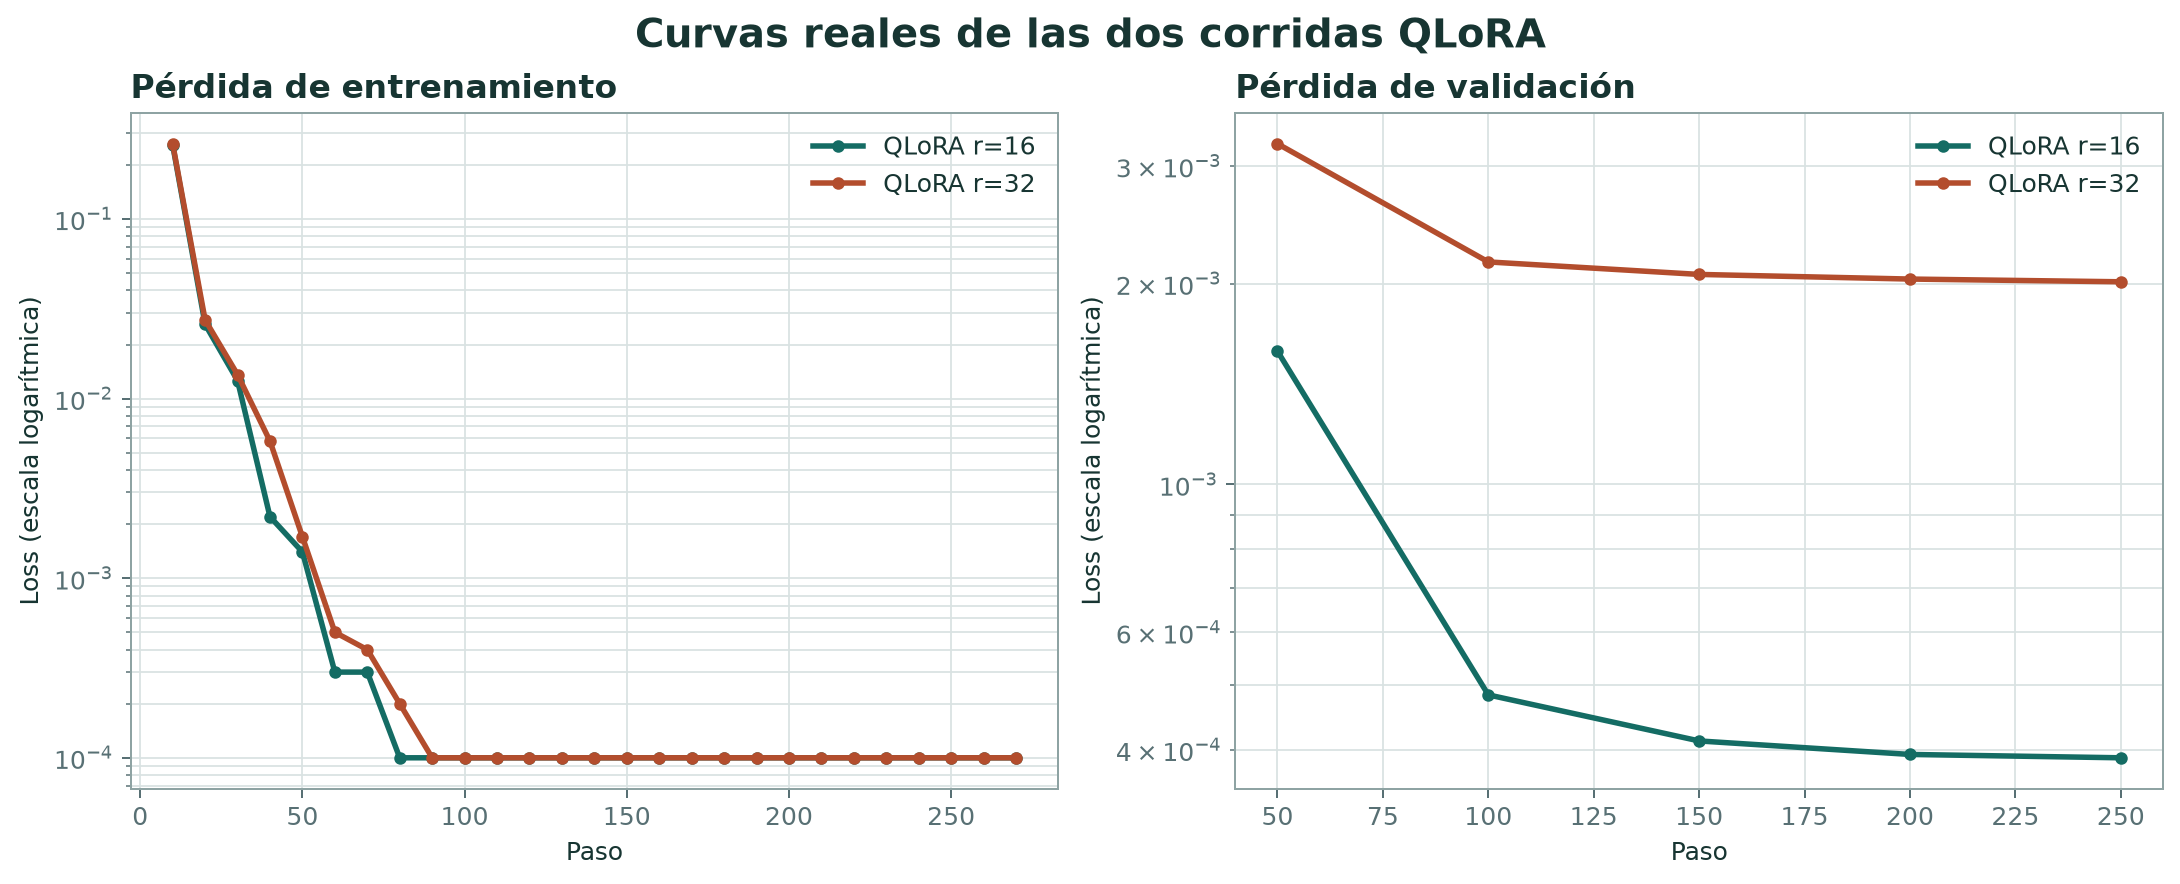
\includegraphics[width=\textwidth]{resultados/curvas_loss.png}
\caption{Curvas reales de entrenamiento y validación exportadas desde los checkpoints finales. El eje vertical usa escala logarítmica. Los valores y hashes de procedencia están versionados en \code{resultados/curvas\_loss.csv} y \code{resultados/curvas\_loss.json}.}
\end{figure}

\subsection{Métrica y reparación}

La EX compara resultados normalizados: redondeo numérico a dos decimales, columnas adicionales permitidas y orden exigido solo cuando el caso lo indica. Las dificultades fácil, media y difícil pesan 1, 2 y 3. Para el ganador se comparó generación directa con una única reparación tras un error real de MySQL.

\section{Resultados}

\begin{table}[H]
\centering
\caption{Resultados sobre 40 preguntas y dos esquemas no vistos.}
\begin{tabular}{@{}lccc@{}}
\toprule
Variante&EX ponderada&Tasa ejecutable&Latencia p95\\
\midrule
Baseline&3.8\%&62.5\%&6.66 s\\
QLoRA $r=16$&97.4\%&97.5\%&15.72 s\\
QLoRA $r=32$&97.4\%&97.5\%&13.20 s\\
Ganador directo&97.4\%&97.5\%&12.68 s\\
Ganador + reparación&97.4\%&97.5\%&15.64 s\\
\bottomrule
\end{tabular}
\end{table}

\begin{table}[H]
\centering
\caption{EX del ganador directo por dificultad.}
\begin{tabular}{@{}lccc@{}}
\toprule
Dificultad&Fácil&Media&Difícil\\
\midrule
EX&100.0\%&92.9\%&100.0\%\\
\bottomrule
\end{tabular}
\end{table}

El ganador resolvió 39 de 40 preguntas. El único fallo fue una entidad inexistente. La taxonomía exigida quedó con estos conteos: sintaxis 0, columna o tabla inexistente 1, \code{JOIN} 0, agregación 0, filtro 0 y resultado distinto 0. La reparación no cambió la EX y añadió latencia, por lo que su utilidad queda limitada a errores de ejecución recuperables, no a correcciones semánticas generales.

La predicción conservadora para la evaluación oculta es 87.4\%, con intervalo estimado de 81.7\% a 90.0\%. Se obtuvo mediante 20,000 remuestras bootstrap por pregunta y una penalización explícita de 10 puntos porcentuales por cambio de dominio. Es una estimación, no una medición del conjunto oculto.

\section{Compatibilidad limpia en Google Colab T4}

La prueba final se ejecutó en un entorno nuevo de Colab con Tesla T4. El notebook \path{notebooks/04_prueba_integral_colab_t4.ipynb} conserva celdas, salidas, versiones y el commit de origen.

\begin{table}[H]
\centering
\caption{Evidencia medida en Tesla T4.}
\begin{tabular}{@{}ll@{}}
\toprule
Comprobación&Resultado\\
\midrule
Entorno&Tesla T4; CUDA 13.0; PyTorch 2.11.0+cu130\\
Carga del adapter&42.728 s; 1.438 GB VRAM asignada\\
Caso fácil&3.442 s; coincidencia con referencia\\
Caso medio&7.507 s; coincidencia con referencia\\
Caso difícil&9.461 s; coincidencia con referencia\\
Callback con reparación&15.225 s; dos llamadas\\
Carga del baseline&8.091 s; 1.202 GB VRAM asignada\\
Configuración final&Adapter restaurado y activo\\
\bottomrule
\end{tabular}
\end{table}

El smoke test del baseline verificó carga, determinismo, formato y tiempo; no se usa como sustituto de la medición MySQL de 40 preguntas. El notebook finaliza con \emph{PRUEBA COMPLETA EN T4 APROBADA}.

\section{Reproducción paso a paso}

\subsection{Ruta autosuficiente de Colab}

\begin{enumerate}
\item Abrir el notebook de prueba y seleccionar \emph{T4 GPU}.
\item Cargar \code{Proyecto-3\_Grupo-1\_DLYSI\_Sec-30-candidato.zip}.
\item Ejecutar todas las celdas en orden.
\item Confirmar el SHA-256 del adapter y el mensaje final de aprobación.
\end{enumerate}

El ZIP ya contiene el adapter; el modelo base público se descarga automáticamente desde Hugging Face. No se requiere token para la ruta normal de evaluación.

\subsection{Recuperación desde Hugging Face}

El modelo base se encuentra en \url{https://huggingface.co/Qwen/Qwen2.5-Coder-1.5B-Instruct}. El respaldo público del adapter está en \url{https://huggingface.co/Dani0604/proyecto3-text2sql-qlora} y se descarga anónimamente, sin token. La revisión fijada es:

\begin{center}
\small\code{24658a4efce8303165906832f0eede2b5c56de84}
\end{center}

Después de descargar, se debe comprobar que \code{adapter\_model.safetensors} tenga SHA-256:

\begin{center}
\small\code{d3126183a092521cb1feffb9424b188552d27bb8fc4b51a8d13a1348d89016f1}
\end{center}

Las instrucciones completas para Colab, Windows, API, Next.js, Docker y recuperación están en \code{README.md}. Las instrucciones de publicación y Git LFS están en \code{docs/PUBLICACION.md}.

\section{Trazabilidad, riesgos y conclusiones}

La entrega incluye configuraciones, adapter, datos, cuatro notebooks, resultados por corrida, revisión humana, bitácora, contribuciones, informe y presentación. MySQL queda fijado en la versión 8.4.10 mediante Docker. La suite automatizada cubre configuración, seguridad SQL, normalización, contrato oficial, API, dataset, auditoría y selección.

El principal riesgo es el cambio de dominio: dos esquemas de validación no representan toda la variedad posible de la prueba oculta. Otros límites son la dependencia de MySQL, la restricción a lectura y la falta de beneficio observado en la reparación. Por ello se reportan EX por dificultad, fallos concretos y una predicción conservadora, sin presentar estimaciones como mediciones.

\begin{resultado}{Conclusión}
El proyecto satisface la ruta experimental exigida: baseline, dos QLoRA que difieren en un factor, evaluación por ejecución, análisis de error, inferencia con reparación, selección justificada, colaboración documentada y prueba limpia en T4. El adapter $r=32$ es el artefacto final por su menor p95 después del empate en calidad.
\end{resultado}

\section*{Uso de inteligencia artificial}

OpenAI Codex apoyó el análisis del enunciado, la implementación, las pruebas y la documentación; v0 se utilizó como punto de partida visual. Los integrantes revisaron los artefactos y son responsables de poder explicarlos. Ninguna API externa participa en la generación SQL evaluada.

\end{document}
